\section{A Laptop-Scale AlphaZero}
\label{sec:system}
\begin{figure}[t]
\centering
% Fig. 1: pipeline diagram (TikZ), included by sections/system.tex
\begin{tikzpicture}[
    box/.style={draw, rounded corners=2pt, align=center, font=\footnotesize, minimum height=0.85cm, inner sep=3pt},
    arr/.style={-{Stealth[length=4pt]}, semithick},
    node distance=0.35cm and 0.6cm]
  \node[box, text width=1.75cm] (self) {Self-play\\(batched PUCT)};
  \node[box, text width=1.35cm, right=of self] (train) {Train\\policy + value};
  \node[box, text width=1.65cm, right=of train] (eval) {Evaluate vs.\\previous gen.};
  \draw[arr] (self) -- (train);
  \draw[arr] (train) -- (eval);
  \draw[arr] (eval.south) |- ++(0,-0.3) -| node[pos=0.25, above=1pt, font=\scriptsize, inner sep=0pt] {next generation} (self.south);
  \node[box, text width=1.3cm, below=1.15cm of self] (py) {Python\\PyTorch};
  \node[box, text width=1.3cm, right=of py] (sw) {Swift app\\Core ML};
  \node[box, text width=1.5cm, right=of sw] (js) {Browser\\ONNX (WASM)};
  \node[draw, dashed, rounded corners=3pt, fit=(py)(sw)(js), inner sep=4pt,
        label={[font=\scriptsize]below:same rules, same search, same network}] {};
\end{tikzpicture}

\caption{One training loop on a laptop CPU; the same rules, search and trained network run in three
runtimes. Chained Elo comes from the ``evaluate vs.\ previous generation'' step.}
\label{fig:pipeline}
\end{figure}

\paragraph{Game and representation.}
We play 9$\times$9 Go with simple ko, no suicide and Tromp--Taylor area scoring (komi 7.5); games end
after two passes or 162 moves. The network sees six planes: each side's stones now and one move ago, the
side to move, and a constant plane.

\paragraph{Network and search.}
A residual network \citep{he2016resnet} with \valNParams{} parameters (Table~\ref{tab:hyper}) outputs move
logits for the 81 points and pass, and a value in $[-1,1]$. Search is PUCT \citep{rosin2011puct} as in
AlphaZero, with one change from Leela Zero: an unvisited move is valued at the parent's value minus a
reduction that grows with the prior probability already explored (first-play urgency).

\paragraph{Self-play and training.}
Ten worker processes each play 16 games in lock step. Every simulation step evaluates one leaf per game in
a single network batch, which keeps a CPU busy without virtual loss or threads. Following KataGo
\citep{wu2019katago}, a quarter of moves receive a full search and become training samples; the rest get a
quarter of the simulations and only advance the game. The network trains with AdamW on a sliding window
of recent positions, with all eight board symmetries, on cross-entropy to the search's visit distribution
plus squared error to the game result. Each generation then plays the previous one in a
\valEvalGames{}-game match at \valEvalSims{} simulations a move; the summed Elo differences form the
chained Elo of the training log.

\begin{table}[t]
\centering
\small
% generated by figures_scripts/hyperparams_table.py
\begin{tabular}{@{}ll@{}}
\toprule
Setting & Value \\
\midrule
Board, komi, move cap & 9$\times$9, 7.5, 162 \\
Input planes & 6 \\
Residual blocks $\times$ channels & 4 $\times$ 48 \\
$c_{\mathrm{puct}}$, FPU reduction & 1.5, 0.25 \\
Dirichlet $\alpha$, $\varepsilon$ & 0.12, 0.25 \\
Sims: full / fast search & 160 / 40 \\
Full-search probability & 0.25 \\
Temperature-1 moves & 10 \\
Games / generation, workers & 160, 10 \\
Batch, learning rate (AdamW) & 256, 0.001 \\
Replay window (positions) & 250,000 \\
Chained eval: games, sims & 40, 32 \\
\bottomrule
\end{tabular}

\caption{Settings of the run, read from the training code and its saved configuration.}
\label{tab:hyper}
\end{table}

\paragraph{Hardware and budget.}
Everything ran on one Intel Core i9-9980HK (8 cores, 16 threads, no GPU). The run took \valNGens{}
generations of \valGamesPerGen{} games each (\valTotalGames{} games, about \valWallHours{} hours of wall-clock
time). That time is approximate: other software shared the machine, and one generation's self-play
took anywhere from \valSelfplayMin{} to \valSelfplayMax{} seconds. Figure~\ref{fig:loss} shows the losses.

\begin{figure}[t]
\centering
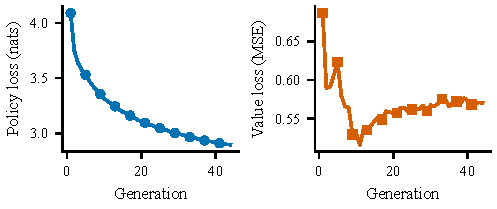
\includegraphics[width=\columnwidth]{figures/loss_curves.pdf}
\caption{Training losses fall steadily across generations: policy cross-entropy from
\valPolicyLossFirst{} to \valPolicyLossLast{} nats, and value MSE from \valValueLossFirst{} to
\valValueLossLast{}. One run.}
\label{fig:loss}
\end{figure}
